\section{Introduction}


The ARTE project is a transient detector receiver working in the frequency range $[1200-1800]$MHz. The aim of this project is to find dispersed signals coming from the galactic center.


The dispersion is a well known electromagnetic effect where a wideband signals have different velocities depending on the frequency.\footnote{If you want the mathematical explanation is in the Griffiths and also in the Pozar}. In our case, the dispersion is produced by the interaction of the electrons that are in the path of the signal, and this is typically expressed with the equations \ref{eq:DM1} where t is the time that one signal is delayed due the interaction with the material in its path, $K_{DM}$ is the so called disperssion constant with value $4.149 GHz2 pc-1 cm3 ms$ and $DM$ is the disperssion measure of the signal that is defined in the equation \ref{eq:DM2}. In the equation \ref{eq:DM2} $n_e$ is the density of electrons, then integrating over the signal path tell us the amount of material that the signal passes through. 

\begin{equation}
    t(f) = DM \cdot K_{DM} \cdot f^{-2} \\
    \label{eq:DM1}
\end{equation}

\begin{equation}
    DM = \int_{path} n_e dl
    \label{eq:DM2}
\end{equation}

In consequence for a given DM value you can have mainly two options that generates this disperssion: 
\begin{itemize}
    \item The signal travels a distance $d$ in a path with the standard electron densities of the universe \footnote{There are models for this number..}.
    \item The signal travels a distance $d'<d$ and passes through an astronomical object that has a higher electron density than the typical one. A simple example is getting a signal when observing in the milky way disk, then this signal had passes through all the material of the galaxy and then it should have a higher DM than the one that you would get if the signal came from higher lattitudes.
\end{itemize}

Then knowing the disperssion measure and with a proper model of the enviroment where the signal has to pass, then you can recover the distance of the object. The figure \ref{fig:dm_example} shows the effect of the interestellar medium (ISM) over a wideband pulse and how it is seen in the earth when receiving it.

\begin{figure}
    \begin{subfigure}{\textwidth}
        \centering
        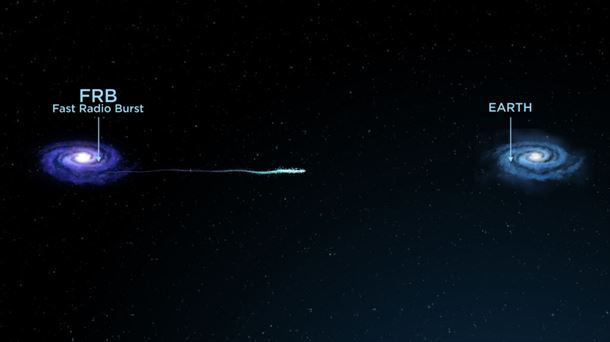
\includegraphics[width=\textwidth, height=0.3\textwidth]{images/frb_example.jpg}
    \end{subfigure}
    \begin{subfigure}{0.5\textwidth}
        %\centering
        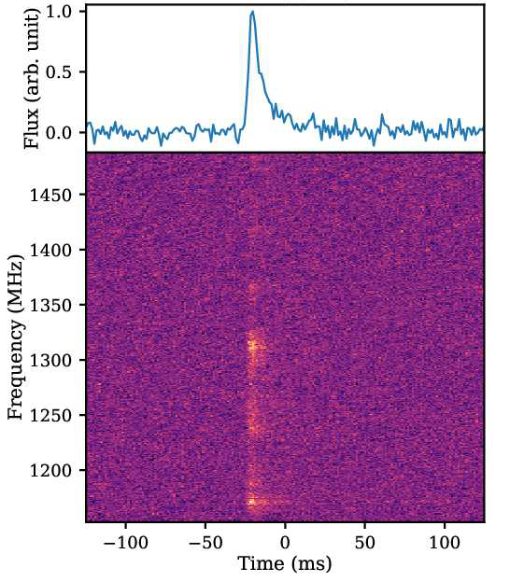
\includegraphics[width=0.5\textwidth]{images/frb_ex_dedispersed.png}
    \end{subfigure}
    \hspace{2cm}
    \begin{subfigure}{0.5\textwidth}
        \centering
        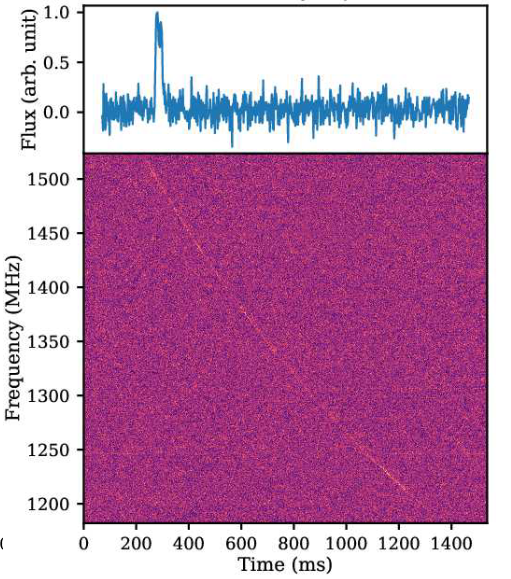
\includegraphics[width=0.5\textwidth]{images/frb_ex_dispersed.png}
    \end{subfigure}
    \caption{This figure depicts the effect of the ISM over the signal. At the source the signal is a wideband pulse and the receipt signal is dispersed in time.}
    \label{fig:dm_example}
\end{figure}








The attention for the astronomical transients was increased with the discover of the Fast Radio Burst, that are strong single pulse signals. The major excitement of this discovery was that when tracing back the distance the astronomers obtained a extragalactic object and the receipt power indicates that the event that produced the signal should be really strong. To this day there are several candidates to be the source of the FRBs but its an on going discussion.

This single pulse signals triggered the design of new types of observation methods. Since the standard telescope has to integrate over long periods to increase the signal-to-noise ratio they are blind to this transient effects and you need a custom made signal processing pipeline that is constantly looking for this events in real time. 


For the ARTE project we decided to use an FPGA as the main driver of the hard real-time constraint, but also sending spectras to be post-processed offline. In the next sections the digital pipeline is described, the technical decisions are explained, some design techniques are presented and suggestions about the drawbacks and possible improvements are presented.


